% =====================================================================
%  IN6049 --- Forecasting and Regression Analysis
%  Week 6: Model Selection and Validation --- Tips dataset
%
%  Built from template/slides-template.tex (Boadilla + seahorse, 16:9).
%  Title slide + 9 content slides.  Numbers come from Assigment_6.ipynb;
%  figures are its exported PNGs (images/ -> fig_*.png here).
%
%  Compiles on Overleaf with the default pdfLaTeX engine.
%  Upload alongside: fig_corr.png , fig_crit.png , fig_mspr.png , fig_smoker.png
% =====================================================================
\documentclass[aspectratio=169,11pt]{beamer}

\usetheme{Boadilla}
\usecolortheme{seahorse}
\setbeamertemplate{navigation symbols}{}

\usepackage[utf8]{inputenc}
\usepackage[T1]{fontenc}
\usepackage{booktabs}
\usepackage{amsmath}
\usepackage{graphicx}
\usepackage{url}

% Emphasis lead-in: bold + structure colour.  Use as \key{Finding.} text...
\newcommand{\key}[1]{\textbf{\structure{#1}}}

% Figure placeholder, so the template compiles with no image files.
% Replace each use by  \includegraphics[width=0.9\linewidth]{@@ file @@}
% (vector PDF preferred; PNG is fine).
\newcommand{\figbox}[2]{%
  \fbox{\parbox[c][#2][c]{#1}{\centering\scriptsize\color{gray}@@ figure @@}}}

% ---------------------------------------------------------------------
\title[Model selection and validation]{Model Selection and Validation --- Restaurant Tips}
\subtitle{Which predictors to keep, and does the model hold up?}
\author[Jie Dong, Elivier Reyes]{Jie Dong, Elivier Reyes}
\date[IN6049]{}

\begin{document}

% ===================== TITLE ========================================
\begin{frame}
  \titlepage
  \vspace{-1.2em}
  \begin{center}
    \small\urlstyle{same}\url{https://github.com/HelloJJJie/Assignment-Forecast-and-Analysis-of-Regression.git}

    \vspace{1.2em}
    $n=244$ restaurant bills, seven candidate predictors --- $2^7=128$ possible
    models. Which one?
  \end{center}
\end{frame}

% ===================== 1. RECAP AND POOL ============================
\begin{frame}{1. Where we start: weeks 1--5 and the candidate pool}
  \begin{columns}[T]
  \begin{column}{0.50\textwidth}
    \small
    \key{What the earlier weeks found} (response: tip):
    \begin{itemize}
      \item The bill alone explains $R^2=0.457$; party size adds little
            ($R^2=0.468$).
      \item Smokers and non-smokers have different bill slopes
            ($0.137$ vs.\ $0.070$): a bill\,$\times$\,smoker interaction.
      \item The variance grows with the bill and the residuals are not normal.
    \end{itemize}

    \vspace{0.3em}
    \key{Notation.} $p$ = number of \emph{parameters} (predictors $+1$); $k=7$
    predictors give $2^k=128$ models, $127$ non-empty subsets.
  \end{column}
  \begin{column}{0.50\textwidth}
    \small
    \key{Seven candidates,} one column each:

    \vspace{0.2em}
    {\scriptsize
    \begin{tabular}{@{}ll@{}}
      \toprule
      \texttt{bill} & total bill (USD) \\
      \texttt{size} & party size \\
      \texttt{smoker}, \texttt{sex}, \texttt{time} & $1=$ smoker / male / dinner \\
      \texttt{weekend} & $1=$ Sat or Sun (\texttt{day} collapsed) \\
      \texttt{bill\_x\_smoker} & \texttt{bill}\,$\times$\,\texttt{smoker} \\
      \bottomrule
    \end{tabular}}

    \vspace{0.4em}
    \small
    \texttt{day} has $4$ classes; collapsing it to \texttt{weekend} keeps every
    candidate a single column, so a subset never splits a qualitative variable.
  \end{column}
  \end{columns}
\end{frame}

% ===================== 2. MODEL BUILDING ============================
\begin{frame}{2. Building a model: fit, parsimony, prediction}
  \begin{columns}[T]
  \begin{column}{0.52\textwidth}
    \small
    More predictors always raise $R^2$ and lower $SSE$, but can overfit and
    inflate variance: the \key{bias--variance trade-off}.

    \vspace{0.3em}
    Process: \key{reduce} the pool (explore, correlations) $\to$
    \key{select} by criteria $\to$ \key{validate} on held-out data.

    \vspace{0.3em}
    \begin{itemize}
      \item Correlation with the tip: bill $0.676$, size $0.489$, then
            bill\,$\times$\,smoker $0.161$, time $0.122$, weekend $0.120$,
            sex $0.089$, smoker $0.006$.
      \item Redundancy to watch: time and weekend $r=0.88$;
            smoker and bill\,$\times$\,smoker $r=0.86$; bill and size $r=0.60$.
    \end{itemize}
  \end{column}
  \begin{column}{0.48\textwidth}
    \centering
    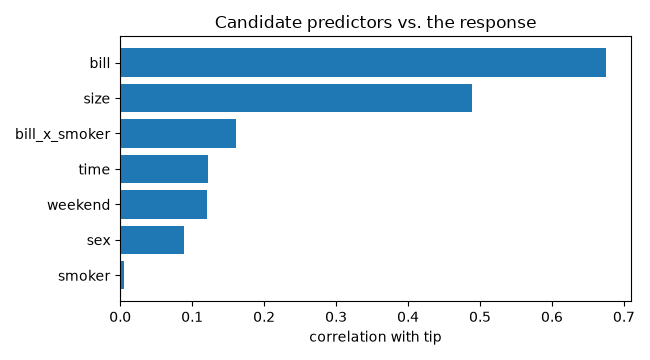
\includegraphics[width=0.92\linewidth]{fig_corr.png}

    \vspace{-0.1em}
    {\scriptsize Smoker alone is almost uncorrelated with the tip, yet it will
     matter through the interaction.}
  \end{column}
  \end{columns}
\end{frame}

% ===================== 3. SIX CRITERIA ==============================
\begin{frame}{3. Six selection criteria}
  \begin{columns}[T]
  \begin{column}{0.56\textwidth}
    \small
    For a model with $p$ parameters:

    \vspace{0.2em}
    {\scriptsize
    \begin{tabular}{@{}lll@{}}
      \toprule
      criterion & formula & choose \\
      \midrule
      $R^2_p$     & $1-SSE_p/SSTO$ & large, always $\uparrow$ \\
      $R^2_{a,p}$ & $1-\frac{SSE_p/(n-p)}{SSTO/(n-1)}$ & maximize \\
      $C_p$       & $\frac{SSE_p}{MSE(F)}-(n-2p)$ & small, $\approx p$ \\
      $AIC_p$     & $n\ln SSE_p-n\ln n+2p$ & minimize \\
      $SBC_p$     & $n\ln SSE_p-n\ln n+p\ln n$ & minimize \\
      $PRESS_p$   & $\sum_i\big(e_i/(1-h_{ii})\big)^2$ & minimize \\
      \bottomrule
    \end{tabular}}
  \end{column}
  \begin{column}{0.44\textwidth}
    \small
    \key{Checked numerically:}
    \begin{itemize}
      \item $C_p=p$ exactly for the full model ($MSE(F)=0.970$).
      \item $PRESS$ from the hat matrix equals an explicit leave-one-out loop.
      \item $R^2_a$ equals \texttt{statsmodels}; its AIC differs from the
            lecture's by the constant $692.44$ for every model --- only
            \emph{differences} matter.
    \end{itemize}
  \end{column}
  \end{columns}
\end{frame}

% ===================== 4. BEST SUBSETS ==============================
\begin{frame}{4. Best subsets: the best model of each size}
  \small
  All $128$ models scored; best model by $SSE$ for each $p$:

  \vspace{0.3em}
  {\scriptsize\setlength{\tabcolsep}{3pt}
  \begin{tabular}{@{}rlrrrrrr@{}}
    \toprule
    $p$ & best subset & $R^2_p$ & $R^2_{a,p}$ & $C_p$ & $AIC_p$ & $SBC_p$ & $PRESS_p$ \\
    \midrule
    1 & (intercept only)                  & $0.000$ & $0.000$ & $237.70$ & $159.5$ & $163.0$ & $469.05$ \\
    2 & bill                              & $0.457$ & $0.454$ & $20.66$  & $12.6$  & $19.6$  & $260.49$ \\
    3 & bill, bill\_x\_smoker             & $0.475$ & $0.471$ & $13.65$  & $6.0$   & $16.5$  & $255.56$ \\
    \textbf{4} & \textbf{bill, smoker, bill\_x\_smoker} & $\mathbf{0.506}$ & $\mathbf{0.4998}$ & $\mathbf{0.97}$ & $\mathbf{-6.6}$ & $\mathbf{7.4}$ & $\mathbf{245.68}$ \\
    5 & + size                            & $0.508$ & $0.4998$ & $2.01$ & $-5.6$ & $11.9$ & $247.98$ \\
    6 & + size, weekend                   & $0.508$ & $0.498$ & $4.00$ & $-3.6$ & $17.4$ & $249.38$ \\
    7 & + size, time, weekend             & $0.508$ & $0.496$ & $6.00$ & $-1.6$ & $22.9$ & $250.50$ \\
    8 & all seven                         & $0.508$ & $0.493$ & $8.00$ & $0.4$  & $28.4$ & $252.27$ \\
    \bottomrule
  \end{tabular}}

  \vspace{0.5em}
  \small
  $p=4$ minimizes $C_p$, $AIC$, $SBC$ and $PRESS$ and maximizes $R^2_{a,p}$;
  $R^2_p$ is flat after it ($0.506\to0.508$). $C_p=0.97\lesssim p$: no detectable bias.
  The full model has $C_p=p=8$ by construction.
\end{frame}

% ===================== 5. CRITERIA PLOT =============================
\begin{frame}{5. All criteria point to the same size}
  \begin{columns}[T]
  \begin{column}{0.62\textwidth}
    \centering
    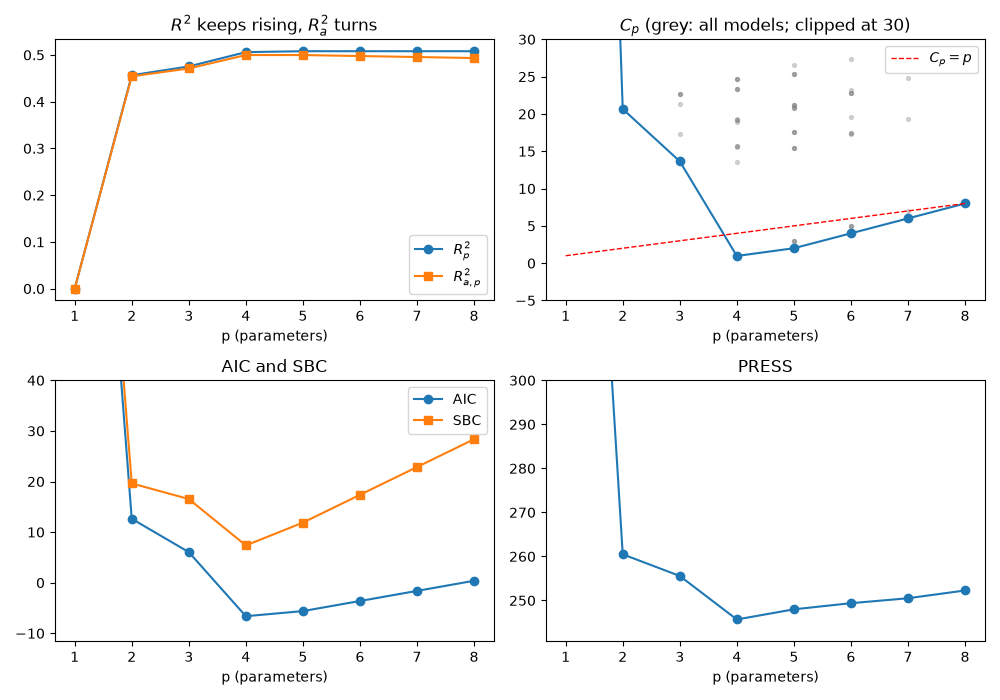
\includegraphics[width=0.94\linewidth]{fig_crit.png}
  \end{column}
  \begin{column}{0.38\textwidth}
    \small
    \begin{itemize}
      \item $R^2$ keeps rising, $R^2_a$ turns after $p=4$.
      \item $C_p$ falls onto the line $C_p=p$ at $p=4$ and then stays on it.
      \item $SBC$ penalizes size more than $AIC$ ($p\ln n$ vs.\ $2p$), so its
            minimum is sharper.
      \item $PRESS$ is lowest at $p=4$: the model predicts best out of sample.
    \end{itemize}
  \end{column}
  \end{columns}
\end{frame}

% ===================== 6. NEAR TIES =================================
\begin{frame}{6. How clear is the winner?}
  \begin{columns}[T]
  \begin{column}{0.56\textwidth}
    \small
    The five best models by $AIC$ (differences from the best):

    \vspace{0.3em}
    {\scriptsize\setlength{\tabcolsep}{3pt}
    \begin{tabular}{@{}lrrrrr@{}}
      \toprule
      adds to bill, bill\_x\_smoker & $p$ & $\Delta AIC$ & $\Delta SBC$ & $R^2_a$ & $C_p$ \\
      \midrule
      + smoker           & $4$ & $0.00$ & $0.00$ & $0.4998$ & $0.97$ \\
      + smoker, size     & $5$ & $1.01$ & $4.51$ & $0.4998$ & $2.01$ \\
      + smoker, time     & $5$ & $2.00$ & $5.50$ & $0.4977$ & $2.97$ \\
      + smoker, weekend  & $5$ & $2.00$ & $5.50$ & $0.4977$ & $2.97$ \\
      + smoker, sex      & $5$ & $2.00$ & $5.50$ & $0.4977$ & $2.97$ \\
      \bottomrule
    \end{tabular}}
  \end{column}
  \begin{column}{0.44\textwidth}
    \small
    \begin{itemize}
      \item The runners-up are the winner plus one useless predictor:
            $\Delta AIC\approx2$ is exactly the penalty for one parameter that
            does not reduce $SSE$.
      \item \texttt{size} comes closest ($\Delta AIC=1.0$, same $R^2_a$): a
            near tie that $SBC$ separates ($\Delta=4.5$).
      \item Choosing $p=4$ is the parsimonious call.
    \end{itemize}
  \end{column}
  \end{columns}
\end{frame}

% ===================== 7. STEPWISE ==================================
\begin{frame}{7. Stepwise regression: three paths, one model}
  \small
  Partial $F$ tests, $\alpha_{enter}=0.05$, $\alpha_{stay}=\alpha_{remove}=0.10$:

  \vspace{0.3em}
  {\scriptsize
  \begin{tabular}{@{}lll@{}}
    \toprule
    Forward selection / forward stepwise & Backward elimination \\
    \midrule
    enter bill \quad $F=203.4$, $P=7\times10^{-34}$ & drop sex \quad $F=0.00$, $P=0.996$ \\
    enter bill\_x\_smoker \quad $F=8.63$, $P=0.004$ & drop time \quad $F=0.00$, $P=0.966$ \\
    enter smoker \quad $F=14.87$, $P=1.5\times10^{-4}$ & drop weekend \quad $F=0.00$, $P=0.950$ \\
    stop: best remaining is size, $P=0.325$ & drop size \quad $F=0.97$, $P=0.325$ \\
     & stop: smoker has $P=1.5\times10^{-4}$ \\
    \bottomrule
  \end{tabular}}

  \vspace{0.5em}
  \begin{itemize}
    \item All three end at \{bill, smoker, bill\_x\_smoker\}, the best-subsets model.
          Forward stepwise never had to drop a term.
    \item Smoker enters \emph{after} the interaction: alone it is uncorrelated with the tip.
    \item Caution: each method explores a single path and the $P$ values are
          optimistic --- best subsets and validation are the check.
  \end{itemize}
\end{frame}

% ===================== 8. VALIDATION ================================
\begin{frame}{8. Validation: data splitting and MSPR}
  \begin{columns}[T]
  \begin{column}{0.54\textwidth}
    \small
    $MSPR=\sum_{i=1}^{n^*}(Y_i-\hat Y_i)^2/n^*$ on the held-out cases, model
    fit on the training half ($122/122$):

    \vspace{0.3em}
    {\scriptsize
    \begin{tabular}{@{}lrrr@{}}
      \toprule
       & $MSE_{train}$ & $MSPR$ & $PRESS/n$ \\
      \midrule
      bill only              & $0.883$ & $1.217$ & $1.068$ \\
      selected (4 parameters) & $0.830$ & $1.126$ & $1.007$ \\
      all 7 predictors       & $0.832$ & $1.186$ & $1.034$ \\
      \bottomrule
    \end{tabular}}

    \vspace{0.3em}
    {\scriptsize One split. Over $1000$ random splits, mean MSPR: bill only
     $1.084$, selected $1.034$, all seven $1.080$.}

    \vspace{0.3em}
    \small
    The selected model has the smallest MSPR in $77\%$ of splits (bill only
    $22\%$, all seven $2\%$).
  \end{column}
  \begin{column}{0.46\textwidth}
    \centering
    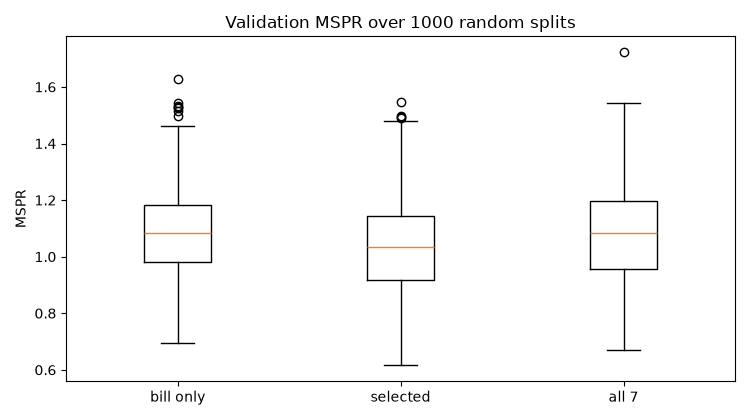
\includegraphics[width=0.94\linewidth]{fig_mspr.png}

    \vspace{-0.1em}
    {\scriptsize MSPR exceeds the training MSE for every model, but the ranking
     is stable.}
  \end{column}
  \end{columns}
\end{frame}

% ===================== 9. SELECTED MODEL ============================
\begin{frame}{9. The selected model and what it leaves open}
  \begin{columns}[T]
  \begin{column}{0.50\textwidth}
    \small
    $\hat Y=0.360+0.1372\,\mathrm{bill}+1.204\,\mathrm{smoker}-0.0676\,\mathrm{bill}\!\times\!\mathrm{smoker}$

    \vspace{0.3em}
    {\scriptsize
    \begin{tabular}{@{}lrrrr@{}}
      \toprule
       & $b$ & $s\{b\}$ & $t^{*}$ & $P$ \\
      \midrule
      intercept     & $0.360$  & $0.202$ & $1.78$  & $0.076$ \\
      bill          & $0.1372$ & $0.0097$ & $14.17$ & $<10^{-32}$ \\
      smoker        & $1.204$  & $0.312$ & $3.86$  & $1.5\times10^{-4}$ \\
      bill$\times$smoker & $-0.0676$ & $0.0142$ & $-4.76$ & $3.3\times10^{-6}$ \\
      \bottomrule
    \end{tabular}}

    \vspace{0.3em}
    $R^2=0.506$, $R^2_a=0.4998$, $MSE=0.958$.
    \begin{itemize}
      \item Slopes: $0.137$ (non-smokers), $0.070$ (smokers).
      \item \key{Still open:} Breusch--Pagan $\chi^2=102.6$ ($P=4\times10^{-22}$)
            and probability-plot $r=0.975$: variance and normality remain
            problems, so intervals for new tips are too narrow at high bills.
    \end{itemize}
  \end{column}
  \begin{column}{0.50\textwidth}
    \centering
    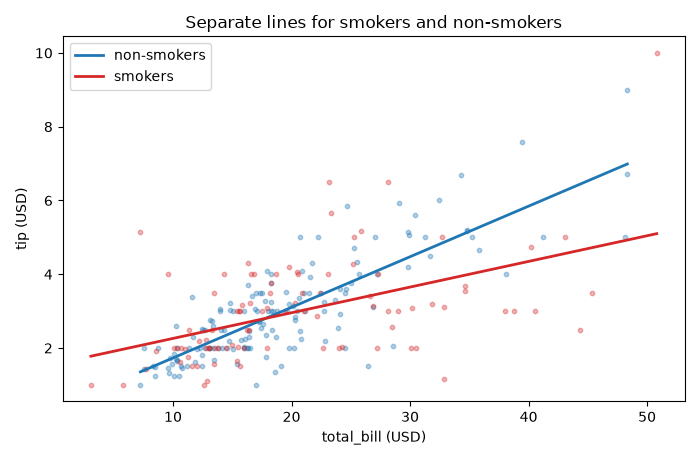
\includegraphics[width=0.92\linewidth]{fig_smoker.png}

    \vspace{0.3em}
    \raggedright\small
    \key{Takeaway.} Every criterion, three stepwise paths and the validation
    agree: of seven candidates, only the bill, smoking status and their
    interaction are needed. Selection does not repair the residuals.\par
  \end{column}
  \end{columns}
\end{frame}

\end{document}
